\selectlanguage{ngerman}%
\frenchspacing%
\begin{ledgroupsized}[r]{120mm}%
\footnotesize%
\pstart%
\noindent%
\textbf{Überlieferung:}%
\pend%
\end{ledgroupsized}%
\begin{ledgroupsized}[r]{114mm}%
\footnotesize%
\pstart%
\parindent -6mm%
\makebox[6mm][l]{\textit{L}}%
Aufzeichnung:
LH XXXVII\;4, Bl.\;151.
Ein Blatt 4\textsuperscript{o},
zum Teil unregelmäßig beschnitten.
Eine Seite auf Bl.\;\href{\Scan{LH_37_04_151r}}{151\,r\textsuperscript{o}};
auf Bl.\;\href{\Scan{LH_37_04_151v}}{151\,v\textsuperscript{o}} Kostenaufstellung,
die vermutlich von Leibnizens Diener und Kutscher Hans%
\indexN{Hans, Leibnizens Diener und Kutscher}
verfasst wurde:
\edlabel{LH_37_04_151_151v_hans-1}%
\textit{Speicifications was ich Behuff außzugeben}
[/]
\textit{erste Nacht ins hauß geschlossen 14 gr.}
[/]
\textit{Zu den schwartzen Bandt 24 gr.}
[/]
\textit{fur wein 2\:\texttt{''}}
[/]
\textit{Zu den Dublüre unter Konsohl 1 gr. 4} \textlangle\textit{pf.}\textrangle\
[/]
\textit{Kasten undt Laden herzuführen 8\:\texttt{''}}
[/]
\textit{1 Thlr 13 gr.} \textlangle\textit{4 pf.}\textrangle\
[/]
\textit{Hanß}%
\edlabel{LH_37_04_151_151v_hans-2}%
\pend%
\end{ledgroupsized}%
\selectlanguage{latin}%
\frenchspacing%
\vspace{8mm}%
\normalsize%
\pstart%
\noindent%
\lbrack%
\href{\Scan{LH_37_04_151r}}%
{151\,r\textsuperscript{o}}%
\rbrack\
\edlabel{LH_37_04_151_151r-annahme-1}%
\edtext{%
In Libra parium brachiorum%
\indexS{libra parium brachiorum}%
\indexS{brachium librae}%
}{%
\lemma{Libra parium brachiorum}%
\Cfootnote{%
Vgl. das Diagramm \lbrack\textit{Fig.\;1}\rbrack.%
}}
\edtext{%
\textit{AB}, \textit{AC}%
}{%
\lemma{\textit{AB}, \textit{AC}}%
\Bfootnote{\textit{erg.\;L}%
}}
sint in aequilibrio%
\indexS{aequilibrium in libra}%
\indexS{pondus aequilibratum}
pondus \textit{D} %
et
\edtext{%
vas \textit{E} aquam continens,%
\indexS{vas continens aquam}%
\indexS{aqua in vase}%
}{%
\lemma{vas \textit{E}}%
\Bfootnote{%
\textit{(1)}~cum liquore %
\textit{(2)}~aquam continens,%
~\textit{L}%
}}
in qua natat%
\indexS{vasculum natans}
\edtext{%
aliud vasculum \textit{F} ex materia%
}{%
\lemma{aliud}%
\Bfootnote{%
\textit{(1)}~vas %
\textit{(a)}~plumbeum\indexS{vas plumbeum} %
\textit{(b)}~\textit{F} ex materia %
\textit{(2)}~vasculum \textit{F} ex materia%
~\textit{L}%
}}
in aqua subsidente,%
\indexS{materia subsidens in aqua}
sed ob
\edtext{%
cavitatem vacuam sustentata.%
\indexS{cavitas vacua}%
\indexS{materia sustentata cavitate vacua}
Sit%
}{%
\lemma{cavitatem}%
\Bfootnote{%
\textit{(1)}~sustentata. Sit %
\textit{(2)}~vacuam sustentata. Sit%
~\textit{L}%
}}
in
\edtext{%
imo vasculi%
}{%
\lemma{imo}%
\Bfootnote{%
\textit{(1)}~vasis %
\textit{(2)}~vasculi%
~\textit{L}%
}}
foramen charta%
\indexS{foramen vasculi obturatum}%
\indexS{charta obturans foramen}
si placet
vel simila aliqua materia obturatum,%
\indexS{materia obturans foramen}
quae initio aquam excludat,%
\indexS{materia excludens aquam} %
paulatim vero transmittat.%
\indexS{materia transmittens aquam}
Ubi ergo aqua vasculum impleverit,%
\indexS{aqua implens vasculum}%
\indexS{vasculum impletum aqua}
descendet;
et durante descensu vasculi \textit{F},%
\indexS{vasculum descendens in aqua}%
\indexS{descensus vasculi in aqua}
cum pondus ejus non amplius%
\indexS{pondus vasculi natantis}
\edtext{%
sustineatur a vase \textit{E} %
neque adeo a pondere \textit{D},
descendet pondus \textit{D}%
\indexS{pondus descendens in libra} %
et ascendet vas \textit{E},
donec vasculum \textit{F} fundum attigerit;
quo facto ad aequilibrium redibitur.%
\indexS{aequilibrium in libra}%
\indexS{reditus ad aequilibrium}%
\edlabel{LH_37_04_151_151r-annahme-2}%
}{%
\lemma{sustineatur}%
\Bfootnote{%
\textit{(1)}~a pondere \textit{D}, vincet hoc pondus %
\textit{(2)}~a vase \textit{E} %
\lbrack...\rbrack\ ascendet vas %
\textit{(a)}~\textit{F} %
\textit{(b)}~\textit{E} donec %
\textit{(aa)}~ad aequi %
\textit{(bb)}~vasculum \textit{F} %
\lbrack...\rbrack\ ad aequilibrium %
\textit{(aaa)}~pervenietur. %
\textit{(bbb)}~redibitur.%
~\textit{L}%
}}
\pend%
\pstart%
\edlabel{LH_37_04_151_151r_anspiel-1}%
Hinc colligitur causa paradoxi,%
\indexS{causa paradoxi}%
\indexS{paradoxon}
cur aer pluvius sit%
\indexS{aer pluvius}
\edtext{%
levior%
\indexS{aer levior}
nec amplius cum barometro%
\indexS{barometrum}
aequilibrium faciat,%
\indexS{aequilibrium aeris et barometri}
\edtext{%
\edlabel{LH_37_04_151_151r_anspiel-3}%
a viris quibusdam egregiis%
\indexS{vir egregius}
jam subindicata,%
\indexS{causa subindicata}
sed non satis dilucide exposita.%
\indexS{causa exposita}%
\edlabel{LH_37_04_151_151r_anspiel-2}%
}{%
\lemma{a viris \lbrack...\rbrack\ exposita}%
\Cfootnote{%
Wohl Anspielung auf B.\;\textsc{Ramazzini}, \textit{Ephemerides barometricae} %
(Modena 1695;\cite{01516} Augsburg 1696).\cite{01517}
Ramazzini\indexN{\textls{Ramazzini} (Ramazzinus), Bernardino 1633\textendash1714} erörtert dort verschiedene Erklärungen des "Paradoxons" %
(1695, S.\;31\,ff.; 1696, S.\;12\,ff.) und schlägt seine eigene vor (1695, S.\;47\,ff.; 1696, S.\;18\,ff.); auch die anschließend abgedrückten Briefe von
\textsc{G.\,B.\;Boccabadati}\indexN{\textls{Boccabadati} (Boccabadatus), Giovan Battista 1635\textendash1696} (1695, S.\;77--87; 1696, 31--36)\cite{01465} und 
\textsc{F.\;Torti}\indexN{\textls{Torti} (Tortus), Francesco 1658\textendash1741} (1695, S.\;89--127; 1696, S.\;37--60)\cite{01519} gehen auf das Phänomen ein.
Unter den von Ramazzini dargelegten Erklärungen sind vornehmlich zwei (1695, S.\;31\,f., 38;\cite{01516} 1696, S.\;12\,f.,\;15)\cite{01517} mit Leibnizens Ansatz verwandt:
die eines "autor anonymus"\indexN{\textls{Alencé} (d'Alancé, Dalancé, Dalancay, Dalencé), Joachim de 1640\textendash1707} (\textsc{J.\;d'Alencé}, \textit{Traittez des baromètres}, Amsterdam 1688,\cite{01525} S.\;45\,f.)
und diejenige von C.\;Comiers\indexN{\textls{Comiers}, Claude, gest. 1693} (nach \textsc{P.\;Le Lorrain de Vallemont}, \textit{Physique occulte}, cap.\;XI, Paris 1693,\cite{01513} Bd.\;II, S.\;355).\indexN{\textls{Le Lorrain de Vallemont} (Vallemontius), Pierre 1649\textendash1721}
}}%
}{%
\lemma{levior}%
\Bfootnote{%
\textit{(1)}~, quam viri nonnulli docti subinnuerunt etsi e %
\textit{(2)}~nonnullis egregiis jam indicata %
\textit{(3)}~nec amplius %
\lbrack...\rbrack\ aequilibrium faciat, %
\textit{(a)}~jam indicata a %
\textit{(b)}~a viris %
\lbrack...\rbrack\ dilucide exposita.%
~\textit{L}%
}}
\pend%
\newpage%
\pstart%
\noindent%
\lbrack\textit{Nachfolgend kleingedruckter Text in L gestrichen:}\rbrack\
\pend%
\vspace{0.5em}%
\footnotesize%
\pstart%
\noindent%
\edtext{%
Nempe columna aeris \textit{GH}%
\indexS{columna aeris}%
\indexS{aer atmosphaericus}%
}{%
\lemma{columna aeris \textit{GH}}%
\Cfootnote{%
Vgl. das Diagramm \lbrack\textit{Fig.\;2}\rbrack.%
}}
usque ad supremum atmosphaerae aereae%
\indexS{supremum atmosphaerae}%
\indexS{atmosphaera aerea}
\edtext{%
assurgens,
aequilibrium faciet%
\indexS{aequilibrium aeris et hydrargyri}%
\indexS{columna hydrargyri}%
\indexS{hydrargyrum}
cum Hydrargyri columna \textit{LM}. %
Sint autem in aere dispersae
particulae aqueae tam exiguae%
\indexS{particulae aqueae dispersae in aere}%
\indexS{particulae aqueae sine vi descendendi}%
\indexS{vis descendendi}
ut vim descendendi non habeant%
\lbrack,\rbrack\
quamdiu aer aquae particulas in ipso dilatatas sustinet;%
\indexS{aer sustinens particulas aqueas}
ubi vero aqua cadere incipit,%
\indexS{aqua cadens in aere}
non amplius sustinebitur ab aere,%
\indexS{aqua sustenta ab aere}
atque%
}{%
\lemma{assurgens,}%
\Bfootnote{%
\textit{(1)}~et aequilibrium faciens %
\textit{(2)}~aequilibrium faciet cum %
\textit{(a)}~\textit{L} %
\textit{(b)}~Hydrargyri columna \textit{LM} %
\textit{(aa)}~, descendentibus %
\textit{(bb)}~, ubi non amplius sustinebit aquam in ea dispersam et rarefactam\indexS{aqua dispersa in aere}\indexS{aqua rarefacta} %
\textit{(cc)}~. Sint autem in aere dispersae %
\textit{(aaa)}~aquae particulae %
\textit{(bbb)}~particulae aqueae %
\lbrack...\rbrack\ non habeant %
\textit{(aaaa)}~sed sustententur %
\textit{(aaaaa)}~. Eaedem %
\textit{(bbbbb)}~, et quidem ideo quod nimium habent superficiei proportione molis\indexS{proportio superficiei ad molem} %
\textit{(aaaaa-a)}~, atque adeo %
\textit{(bbbbb-b)}~, cumque ipsae %
\textit{(ccccc-c)}~. Cum enim valde tenues et dilatatae[\textit{!}] ajo fieri, ostendendum primum fieri posse ut %
\textit{(bbbb)}~quamdiu %
\textit{(aaaaa)}~sustinet %
\textit{(bbbbb)}~aer aquae %
\lbrack...\rbrack\ dilatatas sustinet; %
\textit{(aaaaa-a)}~sed %
\textit{(bbbbb-b)}~ubi %
\textit{(aaaaa-aa)}~non ampli %
\textit{(bbbbb-bb)}~au %
\textit{(ccccc-cc)}~aqua non amplius %
\textit{(ccccc-c)}~ubi vero aqua cadere incipit, %
\textit{(aaaaaa-aa)}~\textlangle ajo\textrangle\ %
\textit{(bbbbbb-bb)}~non amplius %
\lbrack...\rbrack\ aere, atque%
~\textit{L}%
}}
\lbrack\textit{Text bricht ab.}\rbrack
\pend%
\normalsize%
\begin{edfigure}[3.5em][3.5em]%
\hspace*{-46mm}%
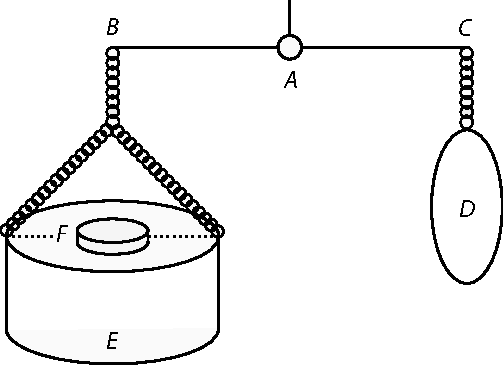
\includegraphics[width=0.55\textwidth]
{gesamttex/edit_VIII-4/images/LH_37_04_151-d1_151r.pdf}%
\edcaption[0.5em]{%
\hspace*{-34mm}%
\lbrack\textit{Fig.\:1}\rbrack%
}%
\vspace{-16.00em}%
\hspace*{86mm}%
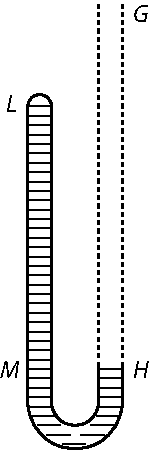
\includegraphics[width=0.156\textwidth]
{gesamttex/edit_VIII-4/images/LH_37_04_151-d2_151r.pdf}%
\edcaption[0.5em]{%
\hspace*{86mm}%
\lbrack\textit{Fig.\:2}\rbrack%
\edtext{%
}{%
\lemma{\lbrack\textit{Fig.\:2}\rbrack}%
\Cfootnote{%
\textit{L} überliefert (Bl.\;\href{\Scan{LH_37_04_151r}}{151\,r\textsuperscript{o}}) drei gestrichene, hier nicht wiedergegebene Entwürfe zum Diagramm.%
}}%
}%
\end{edfigure}%
\selectlanguage{latin}%
\frenchspacing%
\normalsize%
